\documentclass[12pt]{article}

\usepackage[utf8]{inputenc}
\usepackage[a4paper, total={6in, 10in}]{geometry}

\title{Binary Search Trees}
\author{Manuel Serna-Aguilera}
\date{}
\setlength{\parindent}{0pt}

\usepackage{natbib}
\usepackage{graphicx}
\usepackage{amsmath}
\usepackage{clrscode3e}

\begin{document}

\maketitle

\section*{Introduction}
A \textbf{binary search tree} (or bst) is a more organized binary tree. In it each node contains a key value by which it can be searched, additional satellite data, and pointers $\id{left}$, $\id{right}$, and $p$ which point to the left child, right child, and parent node, respectively. The pointers may be populated, otherwise they will have the value NIL (coming form Latin, meaning \textit{nothing}). The root is the top node from which all nodes are descended. 
\\ \\
These keys are stored in such a way that they satisfy the \textbf{\emph{binary-search-tree property}}:

\begin{itemize}
    \item[] Let $x$ be a node in a binary search tree. If $y$ is a node in the left subtree of x, then $\attrib{y}{key} \leq \attrib{x}{key}$. If $y$ is a node in the right subtree of x, then $\attrib{y}{key} \geq \attrib{x}{key}$.
\end{itemize}

Three ways to walk, or traverse, binary search trees:
\begin{itemize}
    \item[]\textbf{Inorder tree walk}: traverse left subtree, visit current node, and then traverse right subtree. 
    \\ \\
    This prints out all keys in sorted order, and traversing every node takes $\Theta{(n)}$ time when starting from the root.
    %--------------------------------------------
    % Inorder tree walk
    %--------------------------------------------
    \begin{codebox}
    \Procname{\proc{inorder-tree-walk}$(x)$}
    \li \If $x \neq \const{NIL}$
    \li \Then
            $\proc{inorder-tree-walk}(\attrib{x}{left})$
    \li     print $\attrib{x}{key}$
    \li     $\proc{inorder-tree-walk}(\attrib{x}{right})$
    \end{codebox}

    \item[]\textbf{Preorder tree walk}: visit current node, traverse left subtree, and traverse right subtree.
    
    %--------------------------------------------
    % Preorder tree walk
    %--------------------------------------------
    \begin{codebox}
    \Procname{\proc{preorder-tree-walk}$(x)$}
    \li \If $x \neq \const{NIL}$
    \li \Then
            print $\attrib{x}{key}$
    \li     $\proc{preorder-tree-walk}(\attrib{x}{left})$
    \li     $\proc{preorder-tree-walk}(\attrib{x}{right})$
    \end{codebox}
    
    \item[]\textbf{Postorder tree walk}: traverse left subtree, traverse
        right subtree, and visit current node.
    
    %--------------------------------------------
    % Postorder tree walk
    %--------------------------------------------
    \begin{codebox}
    \Procname{\proc{postorder-tree-walk}$(x)$}
    \li \If $x \neq \const{NIL}$
    \li \Then
            $\proc{postorder-tree-walk}(\attrib{x}{left})$
    \li     $\proc{postorder-tree-walk}(\attrib{x}{right})$
    \li     print $\attrib{x}{key}$
    \end{codebox}
    
\end{itemize}

\section*{Querying a binary search tree}
Each of the following operations will run in $O(h)$ time for a bst of height $h$. The procedures discussed are, $\proc{search}$, $\proc{minimum}$, $\proc{maximum}$, $\proc{predecessor}$, and $\proc{successor}$.

% figure 12.2
\begin{figure}[!ht]
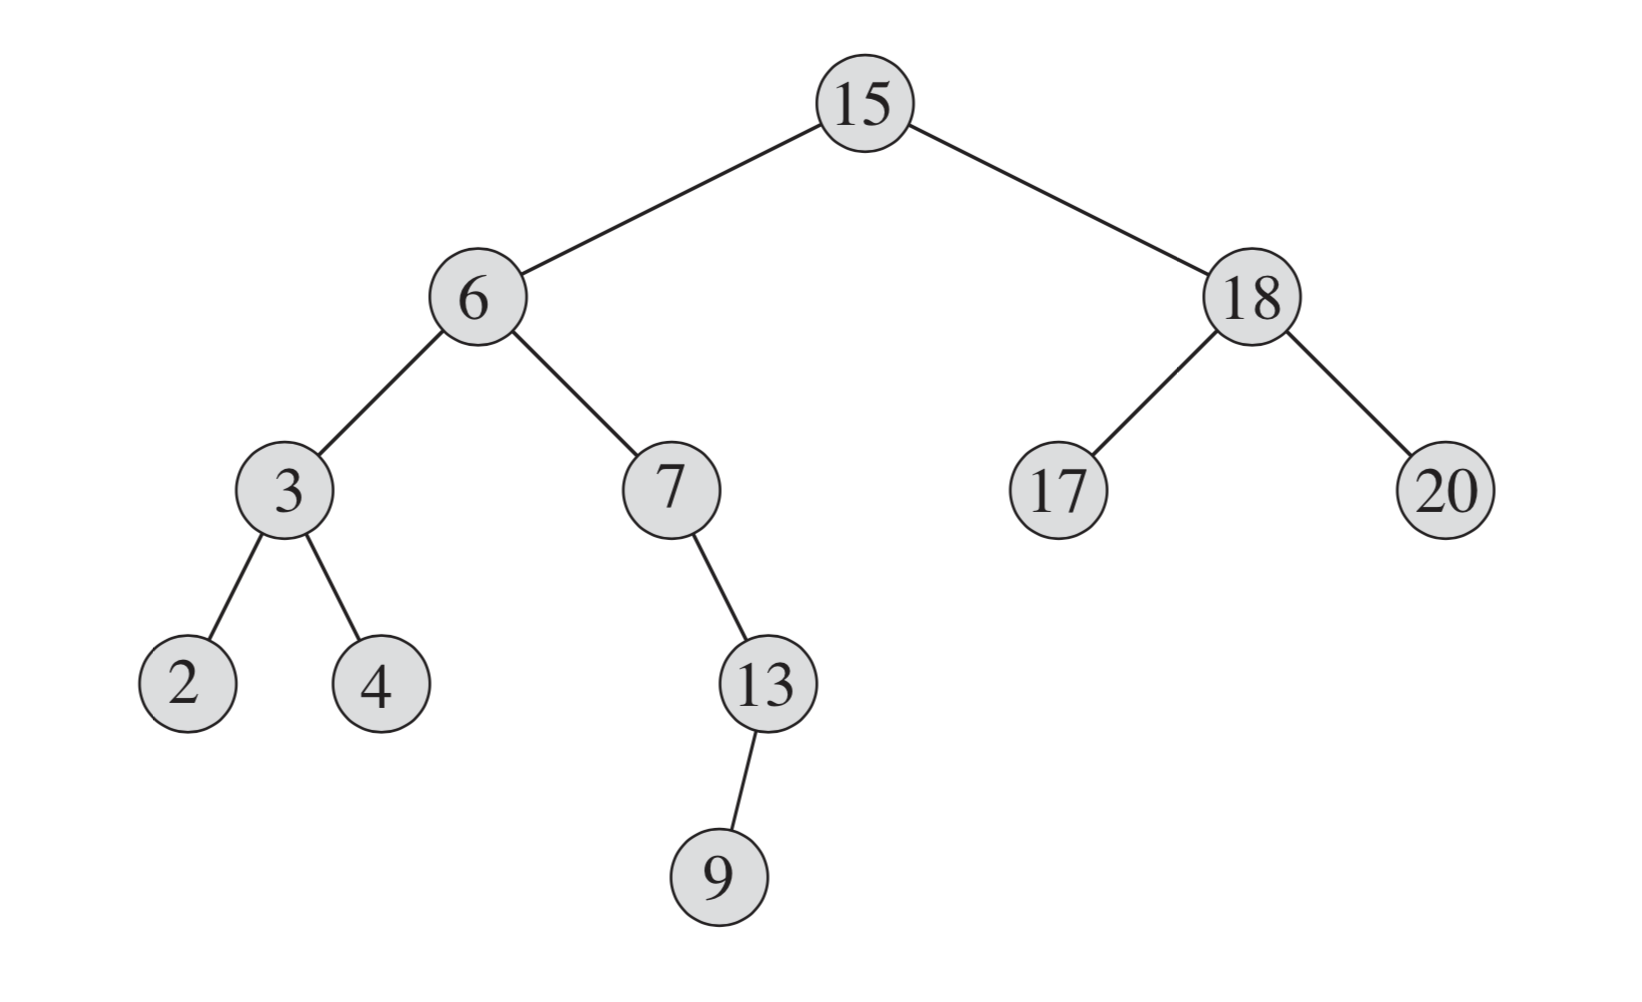
\includegraphics[scale=0.3]{bst1}
\caption{
    Referring to the above binary search tree, here are example cases of queries.
    % search
    \textbf{i.} To \textbf{search} for the lucky number 7, we always start searching at the root (15 at the top). Compare k=7 with the key of the root, $7 < 15$, so go down the \textit{left} subtree. Now compare k=7 with 6, $7 > 6$, so go down the \textit{right} subtree. Now compare k=7 with 7, 7 = 7, duh, so in this simple procedure we return the value 7.
    % minimum
    \textbf{ii.} The \textbf{minimum} key of this bst is 2, you simply follow the \textit{left} pointers.
    % maximum
    \textbf{iii.} The \textbf{maximum} key of this bst is 20, you simply follow the \textit{right} pointers.
    % predecessor
    \textbf{iv.} The \textbf{predecessor} of key 6 is 4, if the node has a left subtree, find the maximum of that left subtree. The predecessor of 9 is 7, if no left subtree exists, simply find the parent of the first node that is a right child (in this case 13 is 7's right child).
    % successor
    \textbf{v.} The \textbf{successor} of 15 is 17, if the node has a right subtree, find the minimum of that subtree. The successor of 13 is 15, if no right subtree exists, simply find the parent of the first node that is a left child (in this case 6 is the right child of 15).
}
\label{fig:bst_example1}
\end{figure}
\newpage

\textbf{Search}
\\ \\
The binary search procedure is straightforward, given a key $k$, we must search the bst for a node with a key that matches $k$. We always start at the root, if $k$ is less than $\attrib{x}{key}$, then we must go down the left subtree, if $k$ is larger than $\attrib{x}{key}$, then we must go down the right subtree, if $k$ is equal to $\attrib{x}{key}$, then we return a pointer to the node $x$. We repeat this process until we find the matching key, otherwise we return NIL.

%--------------------------------------------
% Binary Search
%--------------------------------------------
\begin{codebox}
\Procname{\proc{tree-search}$(x, k)$}
\li \If $x \isequal \const{NIL} \text{ or } k \isequal \attrib{x}{key}$
\li \Then
        \Return $x$
    \End
\li \If $k < \attrib{x}{key}$ 
\li \Then
        \Return $\proc{tree-search}(\attrib{x}{left}, k)$
\li \Else
\li     \Return $\proc{tree-search}(\attrib{x}{right}, k)$
    \End
\end{codebox}

Here is the iterative version, which is more efficient on computers.

%--------------------------------------------
% Iterative Binary Search
%--------------------------------------------
\begin{codebox}
\Procname{\proc{iterative-tree-search}$(x, k)$}
\li \While $x \neq \const{NIL} \text{ and } k \neq \attrib{x}{key}$
    \Do
\li     \If $k < \attrib{x}{key}$ 
        \Then
\li         $x = \attrib{x}{left}$
\li     \Else
\li         $x = \attrib{x}{right}$ 
        \End
    \End
\li \Return $x$
\end{codebox}

\textbf{Minimum and maximum}
\\ \\
Finding the minimum simply means going left on the bst until a NIL value on the $\id{left}$ field is encountered.

%--------------------------------------------
% Minimum
%--------------------------------------------
\begin{codebox}
\Procname{\proc{tree-minimum}$(x)$}
\li \While $\attrib{x}{left} \neq \const{NIL}$
    \Do
    \li     $x = \attrib{x}{left}$
    \End
\li \Return $x$
\end{codebox}

Symmetrically, the right operates in the same manner, but we go all right instead.

%--------------------------------------------
% Maximum
%--------------------------------------------
\begin{codebox}
\Procname{\proc{tree-maximum}$(x)$}
\li \While $\attrib{x}{right} \neq \const{NIL}$
    \Do
    \li     $x = \attrib{x}{right}$
    \End
\li \Return $x$
\end{codebox}

\newpage

\textbf{Predecessor and successor}
\\ \\
Sometimes we want to find the node, based on the inorder tree walk, that comes before or after node $x$. The \textbf{\emph{predecessor}} of a node $x$ is the node with the \textit{largest} key smaller than $\attrib{x}{key}$. 

%--------------------------------------------
% Predecessor
%--------------------------------------------
\begin{codebox}
\Procname{\proc{tree-predecessor}$(x)$}
\li \If $\attrib{x}{left} \neq \const{NIL}$
\li \Then
        \Return $\proc{tree-maximum}(\attrib{x}{left})$
    \End
\li $y = x.p$
\li \While $y \neq \const{NIL}$ and $x \isequal \attrib{y}{left}$
    \Do
        \li $x = y$ 
        \li $y = y.p$
    \End
\li \Return $y$
\end{codebox}

We have two cases to consider when searching for a predecessor.

\begin{enumerate}
    \item If $x$ has a left subtree, find the maximum of that subtree.
    \item If no left subtree exists, find the parent of the first node that is a right child.
\end{enumerate}

The \textbf{\emph{succcessor}} of a node $x$ is the node with the \textit{smallest} key larger than $\attrib{x}{key}$. 

%--------------------------------------------
% Successor
%--------------------------------------------
\begin{codebox}
\Procname{\proc{tree-successor}$(x)$}
\li \If $\attrib{x}{right} \neq \const{NIL}$
\li \Then
        \Return $\proc{tree-minimum}(\attrib{x}{right})$
    \End
\li $y = x.p$
\li \While $y \neq \const{NIL}$ and $x \isequal \attrib{y}{right}$
    \Do
        \li $x = y$ 
        \li $y = y.p$
    \End
\li \Return $y$
\end{codebox}

We have two cases to consider when searching for a successor, which is very much symmetrical to predecessor.

\begin{enumerate}
    \item If $x$ has a right subtree, find the minimum of that subtree.
    \item If no right subtree exists, find the parent of the first node that is a left child.
\end{enumerate}

A good way to remember these procedures is to perform the reverse operations after you think you got the right node.

\newpage

\section*{Insertion}
Inserting a new node into a binary search tree $T$ starts with a binary search in order to find where to insert node $z$, this can be to the left or right of some parent node $y$, or the existing tree may be empty! When we insert $z$, $\attrib{z}{key}$ is some value $v$, while $\attrib{z}{left}$ and $\attrib{z}{right}$ will be NIL. The following procedure will take $O(h)$ time for a tree $T$ of height $h$.

%--------------------------------------------
% Insert
%--------------------------------------------
\begin{codebox}
\Procname{\proc{tree-insert}$(T, z)$}
\li $y = \const{NIL}$
\li $x = \attrib{T}{root}$
\li \While $x \neq \const{NIL}$
    \Do
    \li     $y = x$
        \li \If $\attrib{z}{key} < \attrib{x}{key}$
        \li \Then
                $x = \attrib{x}{left}$
        \li \Else
        \li     $x = \attrib{x}{right}$
            \End
    \End
\li $z.p = y$
\li \If $y \isequal \const{NIL}$
\li \Then
        $\attrib{T}{root} = z$ \Comment tree $T$ was empty
\li \ElseIf $\attrib{z}{key} < \attrib{y}{key}$
\li \Then
        $\attrib{y}{left} = z$
\li \Else
\li     $\attrib{y}{right} = z$
    \End
    
\end{codebox}

\section*{Deletion}
Deleting a node $z$ from a bst $T$ involves three cases, we will reference figure 12.4 from the book.
\begin{itemize}
    \item Node $z$ has no children, remove it from the tree. In terms of pointers, modify the parent so that it refers not to $z$ but $\const{NIL}$ instead (which is the value of $z$'s children).
    \item Node $z$ has one child, replace $z$ with its non-$\const{NIL}$ child. Modify the pointers of the parent and non-$\const{NIL}$ child of $z$ to point "around" it (part (a) and (b) where $l$ is $z$'s left child and $r$ is the right).
    \item Node $z$ has two children, this one is a tad tricky. We replace $z$ with either its predecessor or its successor, but we will go with the successor. There are two cases with this one.
    \begin{itemize}
        \item Right child $r$ is $z$'s successor, in which case we just replace $z$ with $r$.
        \item Right child $r$ is not $z$'s successor, in which case we must find the minimum of the right subtree.
    \end{itemize}
\end{itemize}

\newpage

To move subtrees around, the book defines a neat subroutine called $\proc{transplant}$. This $\proc{transplant}$ procedure replaces the subtree rooted at $u$ with another subtree rooted at a different node $v$, and $u$'s parent becomes $v$'s parent. The pointers to the children of $v$ are not modified, so keep that in mind.

%--------------------------------------------
% Transplant
%--------------------------------------------
\begin{codebox}
\Procname{\proc{transplant}$(T, u, v)$}
\li \If $\attrib{u}{p} \isequal \const{nil}$
\li \Then
        $\attrib{T}{root} \gets{v}$
\li \ElseIf $u \isequal \attrib{u}{\attrib{p}{left}}$
\li \Then
        $\attrib{u}{\attrib{p}{left}} \gets{v}$
\li \Else
\li     $\attrib{u}{\attrib{p}{right}} \gets{v}$
    \End
\li \If $v \neq \const{nil}$
\li \Then
        $\attrib{v}{p} = \attrib{u}{p}$
    \End
\end{codebox}

Having $\proc{transplant}$ defined makes deleting much shorter.
%--------------------------------------------
% Delete
%--------------------------------------------
\begin{codebox}
\Procname{\proc{tree-delete}$(T, z)$}
\li \If $\attrib{z}{left} \isequal \const{nil}$
\li \Then
        $\proc{transplant}(T, z, \attrib{z}{right})$
\li \ElseIf $\attrib{z}{right} \isequal \const{nil}$
\li \Then
        $\proc{transplant}(T, z, \attrib{z}{left})$
\li \Else
\li     $y = \proc{tree-minimum}(\attrib{z}{right})$
\li     \If $\attrib{y}{p} \neq z$
\li     \Then
            $\proc{transplant}(T, y, \attrib{y}{right})$
\li         $\attrib{y}{right} = \attrib{z}{right}$
\li         $\attrib{y}{\attrib{right}{p}} = y$
        \End
\li     $\proc{transplant}(T, z, y)$
\li     $\attrib{y}{left} = \attrib{z}{left}$
\li     $\attrib{y}{\attrib{left}{p}} = y$
    \End
\end{codebox}

The $\proc{tree-insert}$ and $\proc{tree-delete}$ procedure take $O(h)$ time for a bst of height $h$. For insertion, we must perform binary search, which takes $O(h)$ time while rearranging pointers takes constant time. For deletion, everything but $\proc{tree-minimum}$ takes constant time, finding the minimum takes $O(h)$ time again. Figure 12.4 from the book gives a good visualization for the delete cases.

\newpage

% figure 12.4
\begin{figure}[!ht]
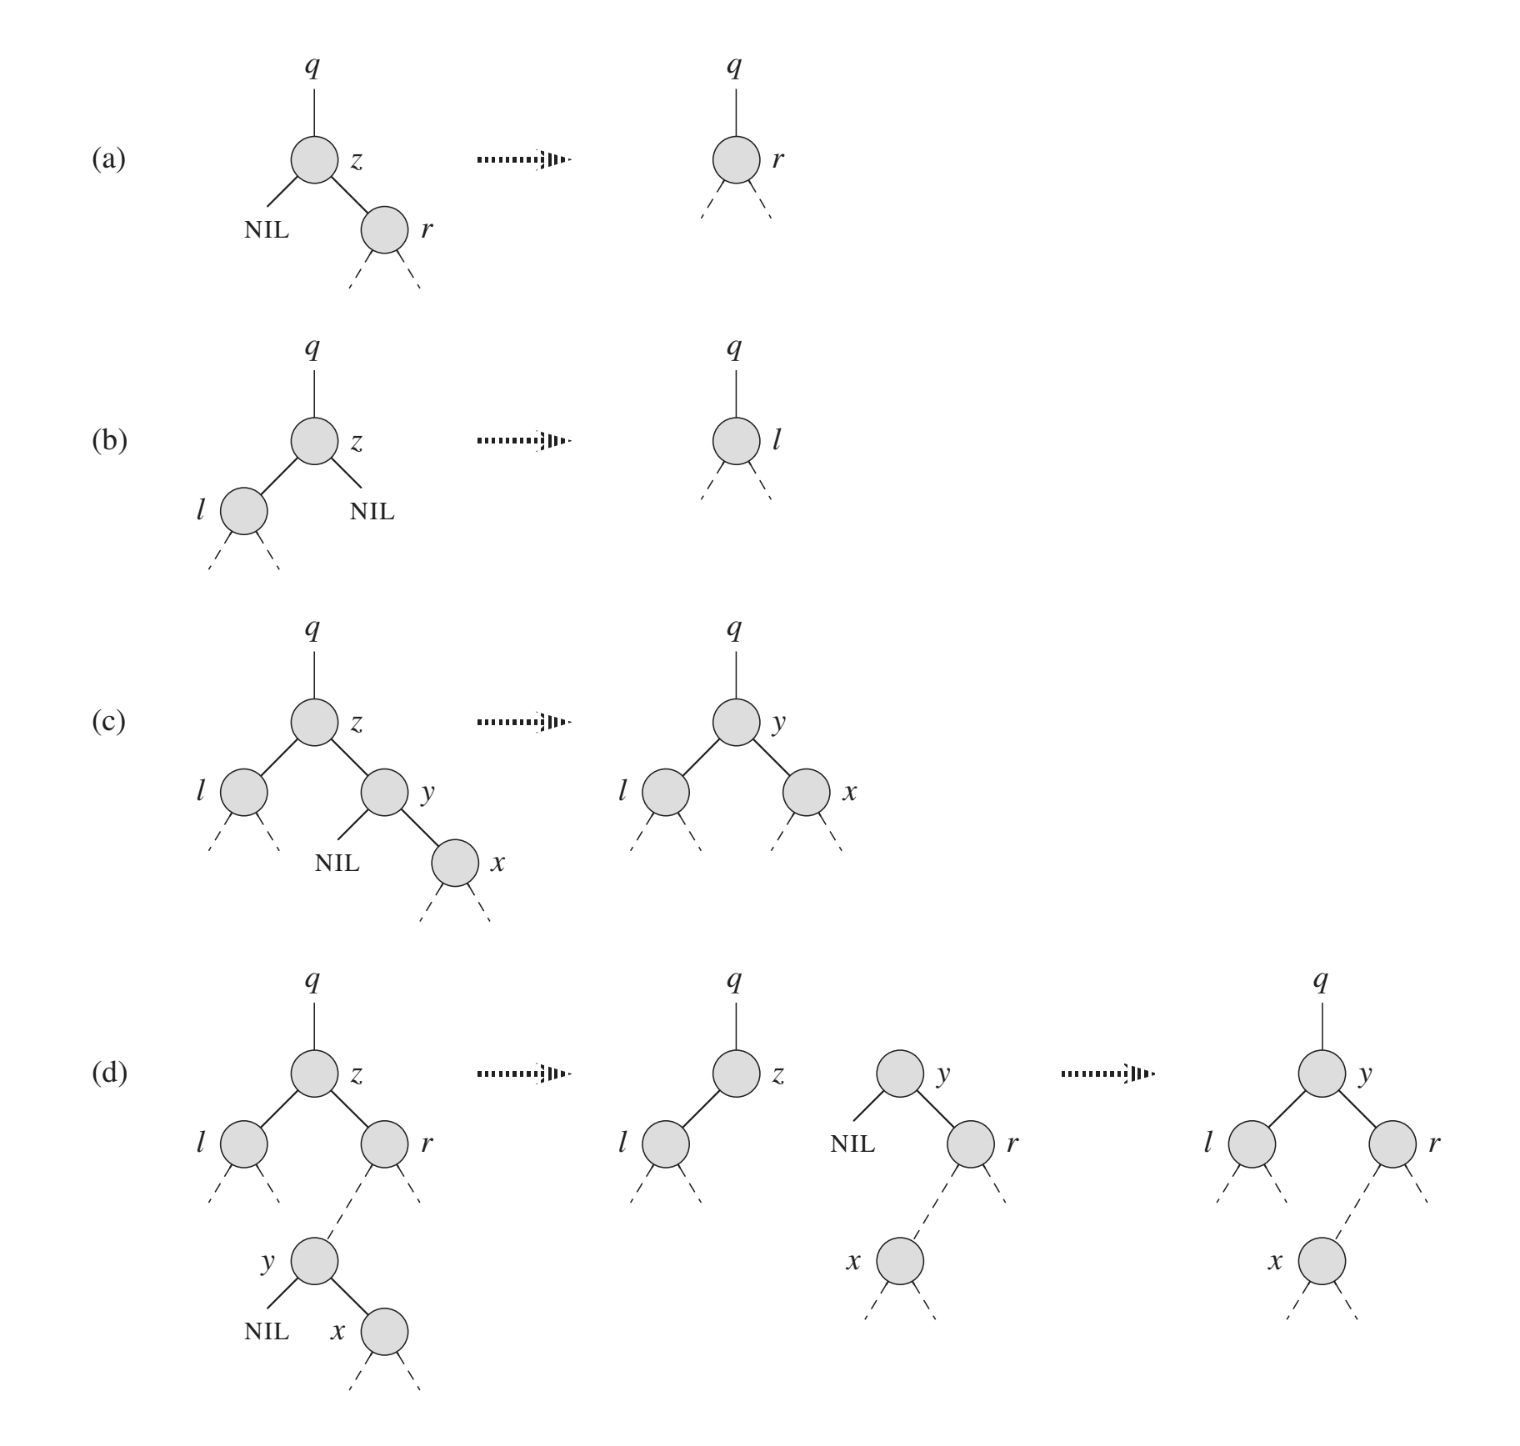
\includegraphics[scale=0.5]{bst_delete_cases}
\caption{
    A visualization of the delete cases.
    \textbf{(a)} shows the single-child case for a right child $r$, and \textbf{(b)} for a left child $l$.
    \textbf{(c)} Two children case, $y$ is $z$'s successor, so replace $z$ with $y$.
    \textbf{(d)} Two children case where $z$'s successor is not its right child, so we must find the smallest key larger than $\attrib{z}{key}$--the minimum of the right subtree.
}
\label{fig:bst_delete}
\end{figure}

\end{document}

